% Лекция по Физике 01.11.2022
% Михедов Константин Константиновчи, БИБ 224

% Тип документа: статья, размер бумаги - A4, написано 14 кегелем
% Предназначено для импорта из другого документа
\documentclass[class=article,a4paper,12pt,crop=false]{standalone}

% Поиск по скомпилированному PDF
\usepackage{cmap}
% Кодировка выходного текста
\usepackage[T2A]{fontenc}
% Кодировка исходного текста
\usepackage[utf8]{inputenc}
% Поддержка необходимых языков
\usepackage[english,russian]{babel}

% Поддержка изображений
\usepackage{graphicx}
\usepackage{graphbox}
% Путь до внешних изображений
%\graphicspath{ {./../figures/}}

% .eps support
\usepackage{epstopdf}
% .svg support
\usepackage{svg}
\usepackage{svg-extract}

% Умная запятая
\usepackage{icomma}

% Ссылки на электронные ресурсы
\usepackage{hyperref}
% Настройка внешнего вида ссылок
\hypersetup{
  % Отключить прямоугольную рамку
  pdfborder={0 0 0},
  % Включить цветные ссылки
  colorlinks=true,
  % Цвет для ссылок на веб-ресурсы
  urlcolor=blue,
  % Цвет внутренних ссылок
  linkcolor=black
}

% Дополнительная математика
\usepackage{amsmath,amsfonts,amssymb,amsthm,mathtools}
% Показывать номера только у тех выржений, на которые кто-то ссылается
\mathtoolsset{showonlyrefs=true}

% Дополнительные символы
\usepackage{mathbbol}

% Подключние пакетов для импорта других .tex
\usepackage[subpreambles=true]{standalone}
\usepackage{import}

\begin{document}
  \subsection{Кинематика}
  \vspace*{.2in}
  \begin{figure}[h]
    \centering
    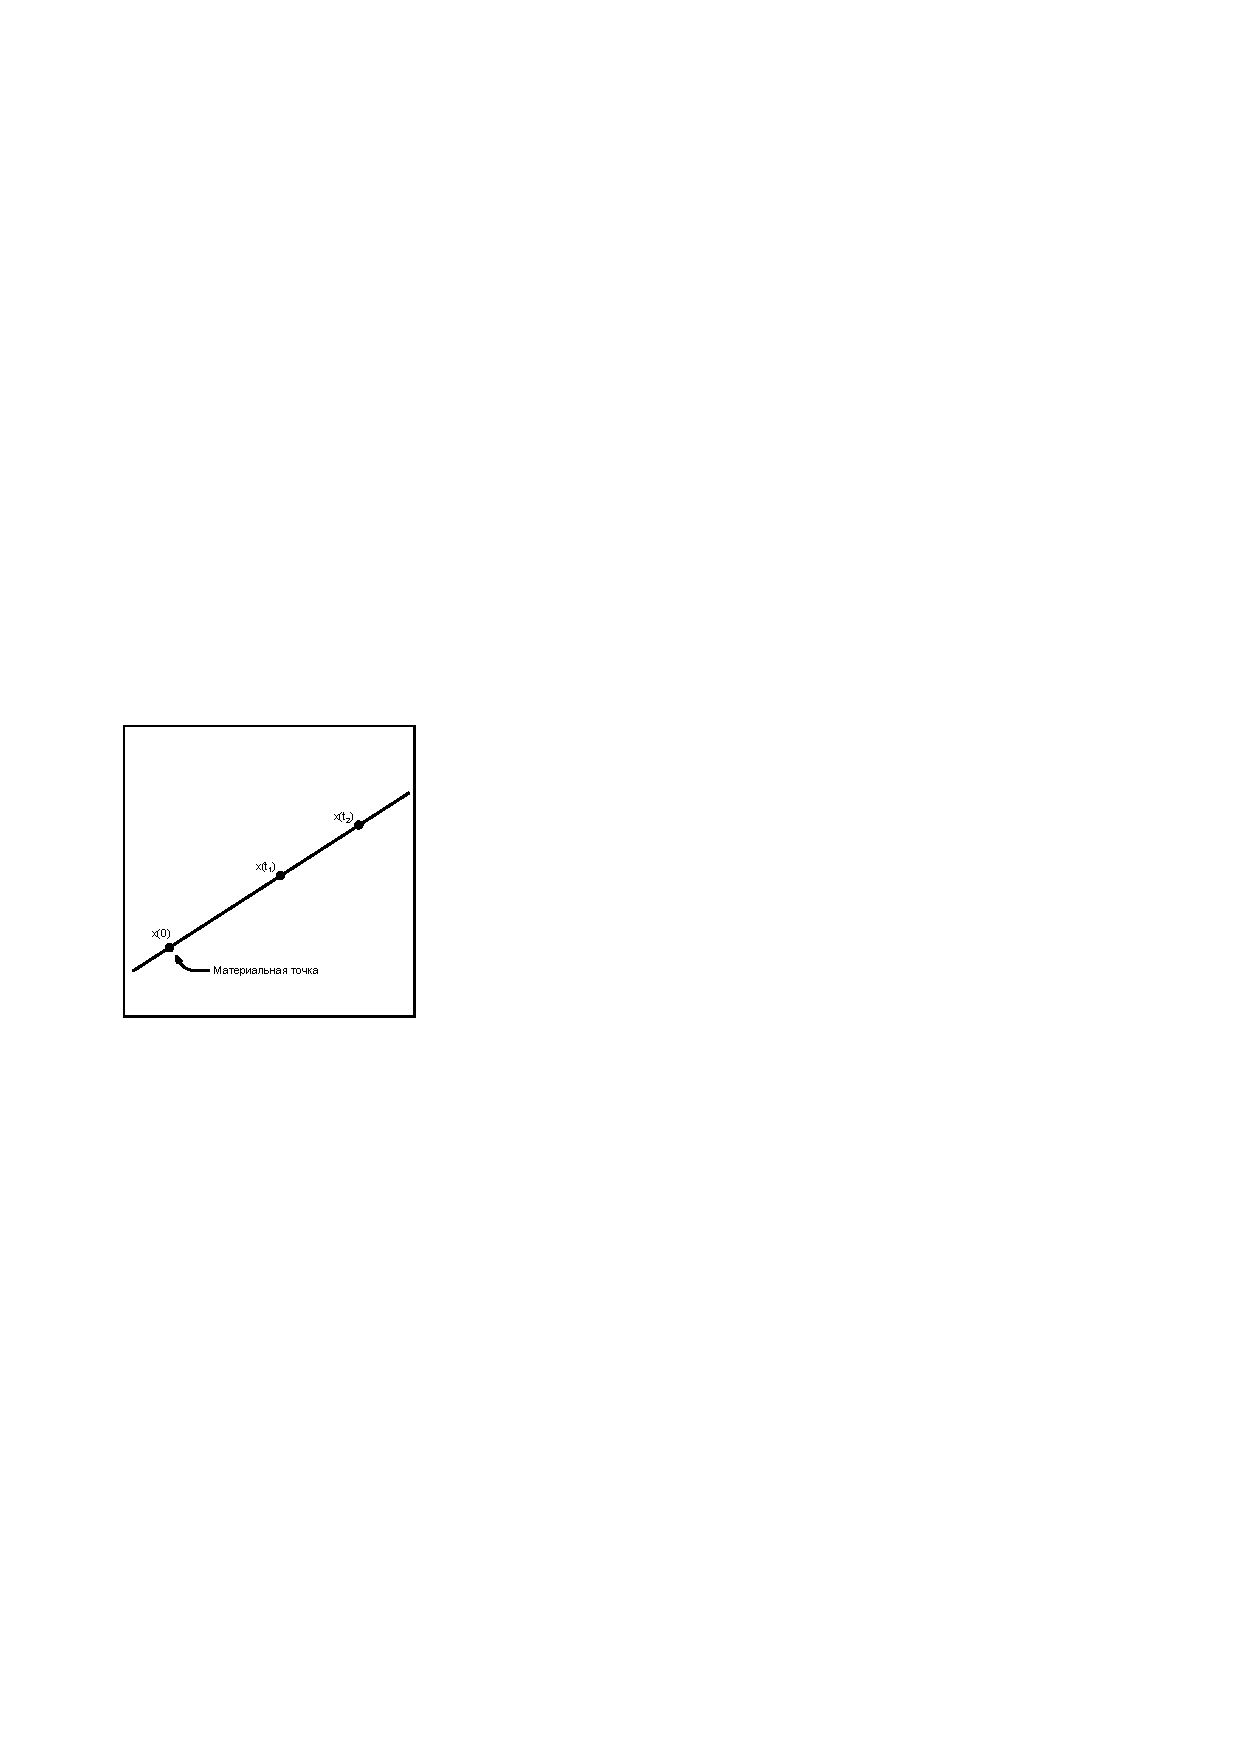
\includegraphics{lec_01_fig_01}
    \hspace*{.5in}
    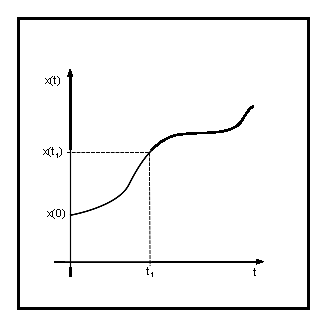
\includegraphics{lec_01_fig_02}
  \end{figure}

  \subsubsection{Скорость}

  \paragraph{Средняя скорость} $<\vartheta > = \frac{x(\tau_2) - x(\tau_1)}{\tau_2 - \tau_1}$

  \paragraph{Мгновенная скорость} $\vartheta(\tau) = \lim\limits_{d\tau \rightarrow 0}\frac{x(\tau + d\tau) - x(\tau)}{d\tau}$

  \subsubsection{Ускорение}

  \paragraph{Среднее ускорение} $<a> = \frac{\vartheta(\tau_2) - \vartheta(\tau_1)}{\tau_2 - \tau_1}$

  \paragraph{Мгновенное ускорение} $a = \lim\limits_{d\tau \rightarrow 0}\frac{\vartheta(\tau + d\tau) - \vartheta(\tau)}{d\tau}$

  \subsubsection{Связь между координатой, скоростью и ускорением}

  \begin{equation}
    \vartheta (\tau) = \frac{dx}{d\tau} = \: \stackrel{\cdot }{x}
  \end{equation}
  \begin{equation}
    a(\tau) = \frac{d\vartheta}{d\tau} = \frac{d^2x}{d\tau^2} = \: \stackrel{\cdot}{\vartheta} = \: \stackrel{\cdot\cdot}{x}
  \end{equation}

  \subsubsection{Равноускоренное движение}

  Равноускоренное движение, это такое, что $a(\tau) = y $ $(y= const)$

  \begin{equation}
    a(\tau) = \frac{d\vartheta}{d\tau} = y \: \Rightarrow \:
    y \times d\tau = d\vartheta \: \Rightarrow \:
    \int y \,d\tau = \int \frac{d\vartheta \times d\tau}{d\tau} = \int a(\tau)\, d\tau
  \end{equation}
  \begin{equation}
    \vartheta(\tau) = y\tau + const \: \stackrel{\vartheta(0) = \vartheta_0 = const}{=} \: y\tau + \vartheta_o
  \end{equation}

  \subsubsection{Сумма Дорбу}

  \begin{figure}[h]
    \centering
    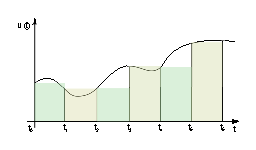
\includegraphics[width=3in, height=1.6in]{lec_01_fig_03}
  \end{figure}  

  \begin{equation}
    \int_o^t \vartheta(t) \, dt = \int_0^t \frac{dx}{dt} \, dt = 
    \sum\limits_{i} \frac{dx}{dt_i} (t_{i + 1} - t_i) 
  \end{equation}

  \subsubsection{Формула Ньютона-Лейбница}

  \begin{equation}
    \int_a^b f(\tau) \, d\tau = \int_a^b \frac{F(\tau)}{d\tau} \, d\tau = F(\tau) |_a^b = F(b) - F(a)
  \end{equation}
  \begin{equation}
    \stackrel{\cdot}{F}(x) = f(x) \text{ то есть } (F(x) \text{ - первообразная})
  \end{equation}

  \subsubsection{Радиус-вектор}

  Положение точки с коордиантами $(x, y)$ можно описать радиус-вектором $\vec{r} = x\vec{i} + y\vec{j}$,
  где $\vec{i} = (1, 0)$, а $\vec{j} = (0, 1)$. Причем $\stackrel{\cdot}{\vec{r}} = \stackrel{\cdot}{x}\vec{i} + \stackrel{\cdot}{y}\vec{j}$

\end{document}
